\newcommand{\DoNotLoadEpstopdf}{}
\documentclass[11pt,a4paper,landscape]{ltjsarticle}
\usepackage[margin=14mm,footskip=7mm]{geometry}
\usepackage{luatexja-fontspec}
\setmainfont{arial.ttf}[Path=C:/Windows/Fonts/,BoldFont=arialbd.ttf]
\setmainjfont{YuGothM.ttc}[Path=C:/Windows/Fonts/,FontIndex=0,BoldFont=YuGothB.ttc,BoldFeatures={FontIndex=0}]
\setsansjfont{YuGothM.ttc}[Path=C:/Windows/Fonts/,FontIndex=0,BoldFont=YuGothB.ttc,BoldFeatures={FontIndex=0}]
\usepackage{graphicx,booktabs,xcolor,amsmath}
\definecolor{ink}{HTML}{263D50}
\setlength{\parindent}{0pt}
\setlength{\parskip}{4pt}
\newcommand{\heading}[2]{{\LARGE\bfseries\color{ink}#1}\par{\small #2}\par\vspace{2mm}}
\begin{document}
\heading{GAの世代が進むと、解同士は似てくるのか}{全ランダムと全CIMの初期集団を新たに比較。各条件16回、300世代を追跡}
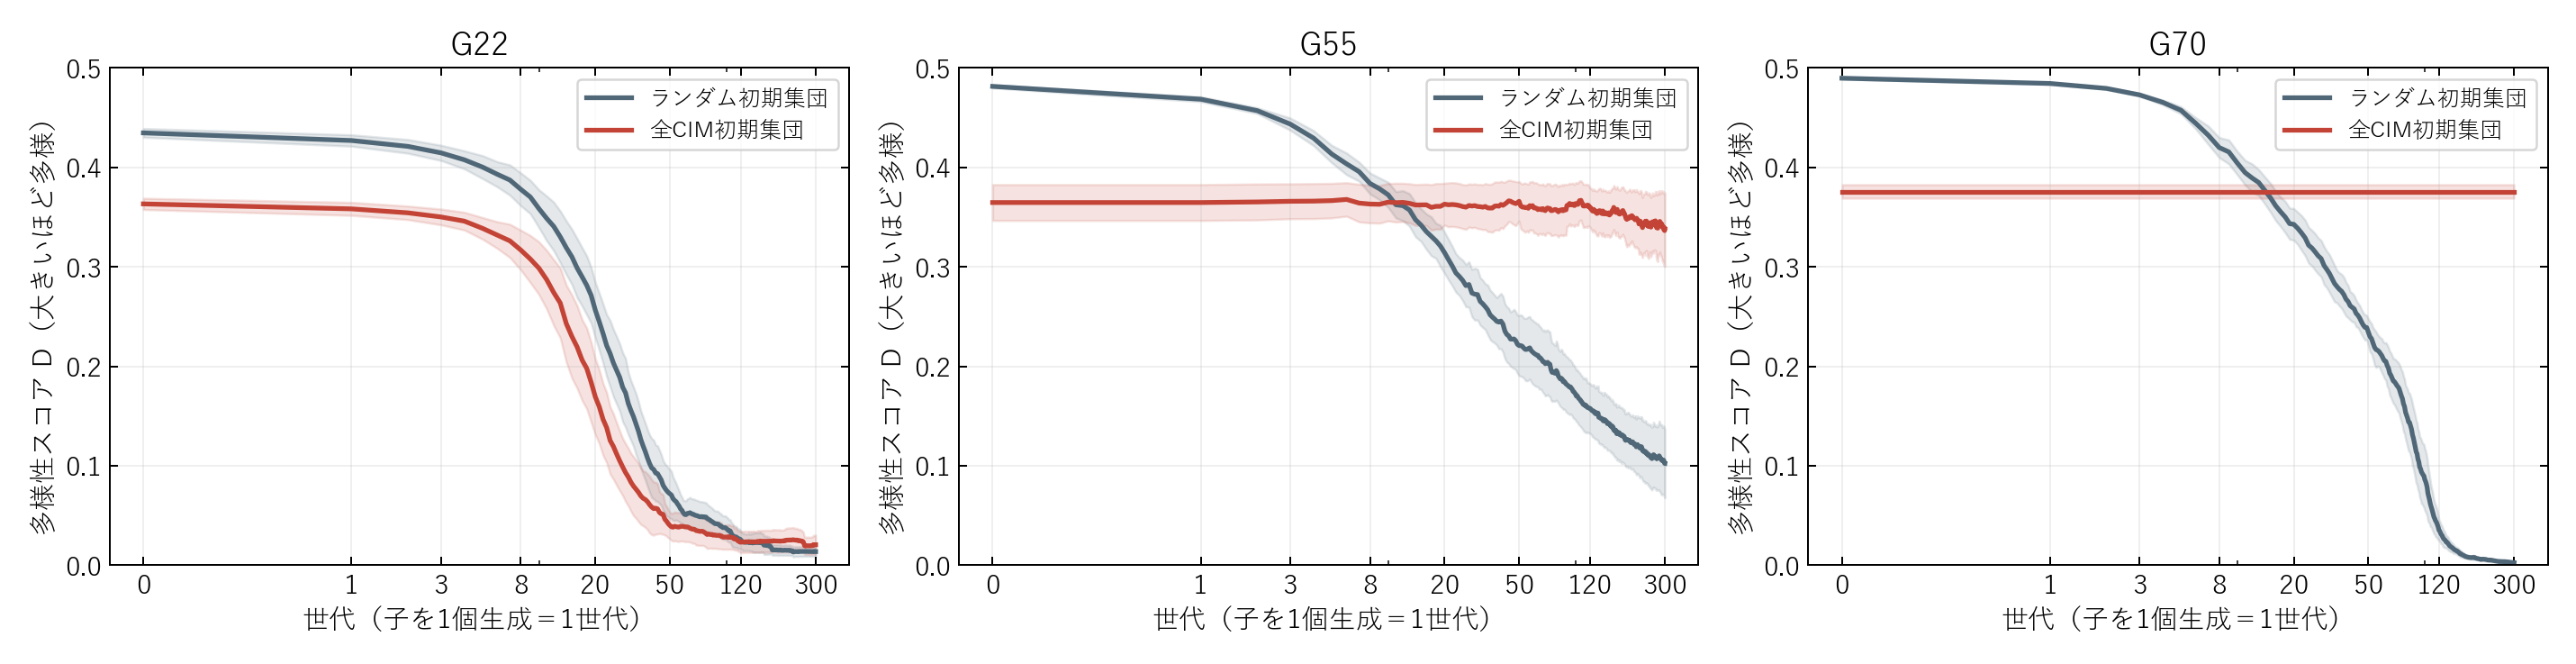
\includegraphics[width=\linewidth,height=85mm,keepaspectratio]{diversity_only.png}

\textbf{線が下がる＝集団内の解同士が似てくる。}スコア$D$は、2解で分け方が違う頂点の割合を集団内の全ペアで平均した値。全反転は同一の解として扱う。$D=0.1$なら平均で10\%の頂点が異なる。

\begin{center}\small
\begin{tabular}{llrrrr}\toprule
問題 & 初期集団 & 初期TS前の$D$ & 世代0の$D$ & 最終世代の$D$ & 最終の異なる分割数\\\midrule
G22 & ランダム & 0.4911 & 0.4345 & 0.0138 & 15.00\\
G22 & 全CIM & 0.3555 & 0.3632 & 0.0207 & 15.00\\
G55 & ランダム & 0.4945 & 0.4813 & 0.1024 & 6.00\\
G55 & 全CIM & 0.3628 & 0.3645 & 0.3380 & 6.00\\
G70 & ランダム & 0.4958 & 0.4895 & 0.0026 & 8.00\\
G70 & 全CIM & 0.3755 & 0.3755 & 0.3755 & 8.00\\
\bottomrule\end{tabular}
\end{center}
{\footnotesize 線はrun平均、帯はrun単位の平均の95\% $t$区間（各世代の区間であり、曲線全体の同時区間ではない）。世代0は初期TS後。異なる分割数はrun平均。}

\clearpage
\heading{多様性の低下と、解の品質を並べて読む}{前ページと同じ実験・同じ世代。最良値は、各runでそれまでに見つけた最良カット値}
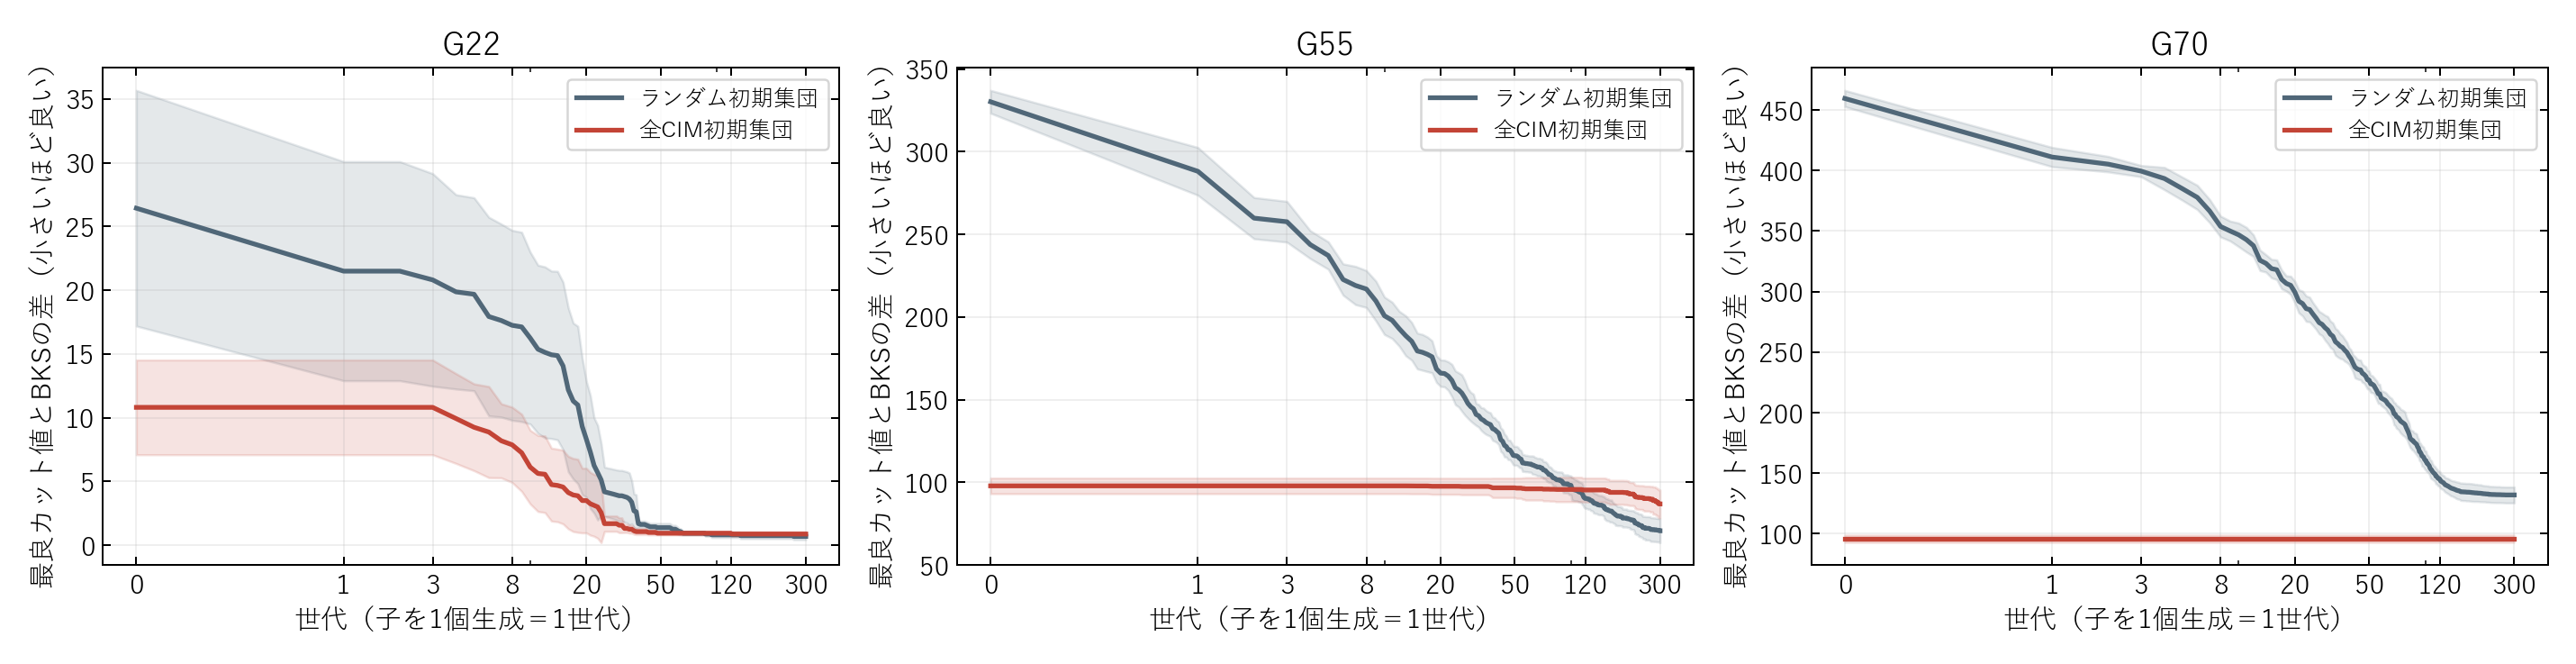
\includegraphics[width=\linewidth,height=85mm,keepaspectratio]{quality_only.png}

\textbf{今回の要点：}G70の全CIM初期集団は、16回すべてで多様性スコアが全世代一定で、最良値も改善しなかった。これは「GA中に多様性を失ったから停滞した」という説明と一致しない。初期の多様性が十分だったかは、別の問いである。

\begin{center}\small
\begin{tabular}{llrrr}\toprule
問題 & 初期集団 & 世代0のBKSとの差 & 最終のBKSとの差 & カット値の改善量\\\midrule
G22 & ランダム & 26.44 & 0.69 & 25.75\\
G22 & 全CIM & 10.81 & 0.88 & 9.94\\
G55 & ランダム & 330.25 & 70.75 & 259.50\\
G55 & 全CIM & 97.94 & 87.00 & 10.94\\
G70 & ランダム & 459.50 & 132.06 & 327.44\\
G70 & 全CIM & 95.81 & 95.81 & 0.00\\
\bottomrule\end{tabular}
\end{center}
{\footnotesize BKSはリポジトリに登録されている既知最良値。表は各runの最良値についての平均。初期品質が異なるため、この比較から多様性が性能差を生んだとは言えない。元のスクリーンショットの実行条件は未確認であり、今回の結果は別の追加実験である。}

\clearpage
\heading{何を測ったか：初期TSと世代更新を区別する}{CIMの生成条件は固定。GAの設定も両初期化条件で同じにした}
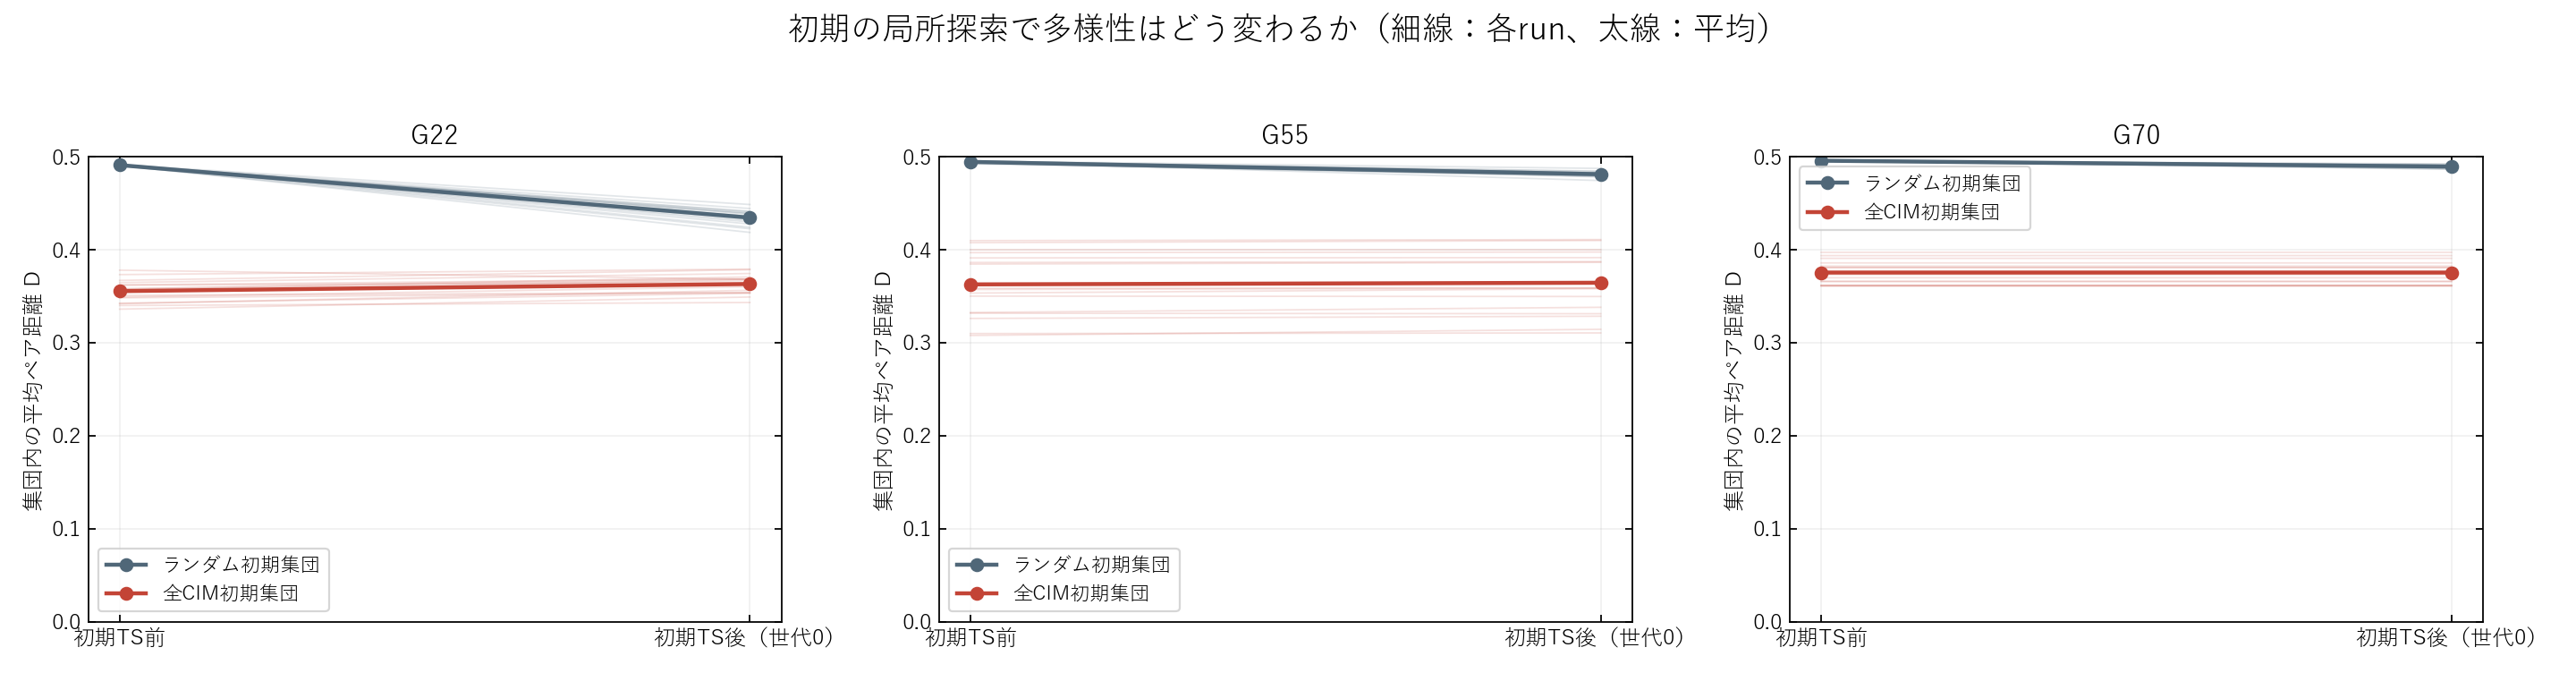
\includegraphics[width=\linewidth,height=77mm,keepaspectratio]{initial_refinement.png}

\textbf{処理の順番：}初期集団を作る $\rightarrow$ 全個体をTabu Searchで改善（ここが世代0）$\rightarrow$ 両親を選ぶ $\rightarrow$ 子を1個作る $\rightarrow$ 子をTSで改善 $\rightarrow$ 集団を更新。最後の4処理を1世代と数える。

集団更新は、カット値と最も近い他個体までの距離を併用するDisQual。したがって、距離が毎世代必ず減るという規則ではない。各runの集団内の多様性を記録し、異なるrunの解を混ぜて計算していない。

\begin{center}\small
\begin{tabular}{lrrrrrr}\toprule
問題 & 集団サイズ & TS反復数 & 摂動待ち回数 & tenure係数 & 品質重み & CIM反復数\\\midrule
G22 & 15 & 35,238 & 2159 & 40 & 0.8374 & 4,800\\
G55 & 6 & 58,453 & 930 & 13 & 0.4330 & 9,600\\
G70 & 8 & 41,152 & 521 & 11 & 0.6618 & 4,800\\
\bottomrule\end{tabular}
\end{center}
{\footnotesize 調整済み設定を使用。CIM解は全個体を独立に新規生成し、品質・距離で選別していない。GAのseedは条件間で対応。CIM生成時間を含めた同一実時間の比較ではない。}

{\footnotesize 検証：864集団の距離と8352個体のカット値を別の計算で照合し、一致を確認。計測でGAの結果が変わらないこと等、7件のテストに成功。全世代の数値、集団の保存断面、設定、seed、コードのハッシュは本PDFと同じフォルダに保存。}
\end{document}
